\documentclass{article} \usepackage{braket} \usepackage{amsmath,amssymb} \usepackage{geometry} \usepackage{graphicx} \usepackage{braket} \usepackage{bm}\usepackage{hyperref} \usepackage{CJKutf8}

\geometry{left=0.5cm,right=0.5cm,top=0.5cm,bottom=0.5cm}

\renewcommand{\theequation}{\arabic{section}.\arabic{equation}} \renewcommand{\baselinestretch}{1.5}
\begin{document}
\begin{CJK}{UTF8}{gbsn}


  \section{Introduction}

  本文主要讲述关于在3D场景中的投影矩阵的构造方法,希望这篇文章可以尽量把两种投影方法讲述清楚明白。

  \subsection{什么是投影矩阵}

  3D场景中的对象,需要显示在屏幕上之前。需要确定场景中哪个区域的的对象显示,并如何显示到屏幕上。也就是需要把3D场景中的一个区域变换为一个正方体区域。然后这个正方体区域和屏幕坐标做一一对应,最终显示在屏幕上。而这个变换过程就叫做投影,相应的变换在数学上被描述为投影矩阵。

  \subsection{两种投影}

  在3D图形学中,有两种最重要和最基本的投影矩阵。一种是正交投影,一种是透视投影。本文也只讲这两种投影的矩阵构建过程。希望帮助大家理解。以下的这张图是直观的感受两种投影矩阵的不同之处。

  \begin{figure}[htbp]
    \centering
    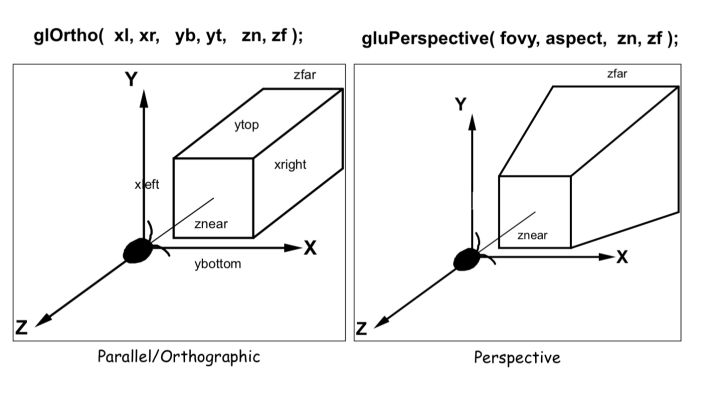
\includegraphics[width=1.0\linewidth]{pic-1.jpg}
  \end{figure}	

  \section{正交投影}

  如何来构建正交投影矩阵?,首先我们来看看正交投影的图像变换过程。如下图。

  \begin{figure}[htbp]
    \centering
    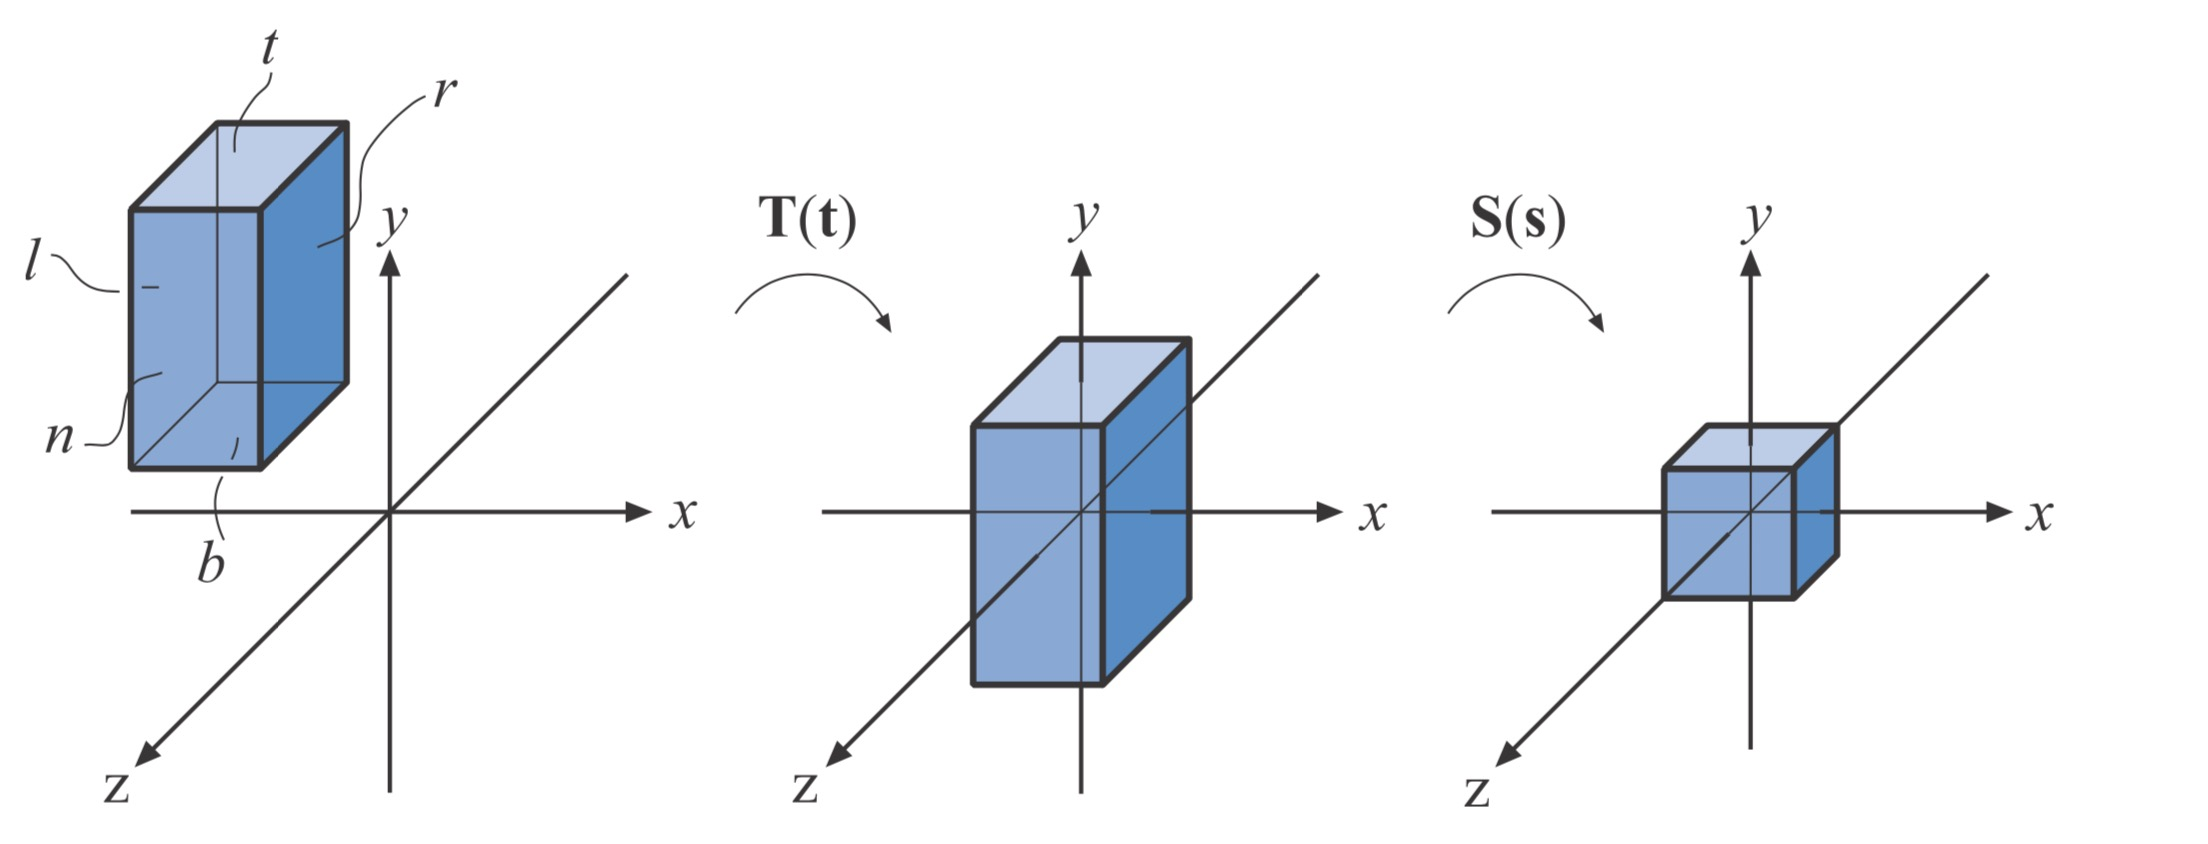
\includegraphics[width=1.0\linewidth]{pic-2.jpg}
  \end{figure}

  如图可以看到,实际上这个过程分为三步。我们在这里列出一张辅助图像作为帮助希望读者更好理解,下面的计算过程
  \begin{itemize}
  \item 第一步,定义显示区域。显示区域的定义为一个长方形区域。这个区域是沿着坐标轴的长方体。
    \begin{displaymath}
      (n_z,f_z,t_y,b_y,l_x,r_y)
    \end{displaymath}
    这个区域就是我们要映射到屏幕坐标的区域。
  \item 将这个区域的中心移动到坐标原点。这一步的矩阵变换简单。我们直接写下。
    \begin{displaymath}
      T(t)=\left(
        \begin{array}{cccc}
          1 & 0 & 0 & -\frac{l+r}{2} \\
          0 & 1 & 0 & -\frac{t+b}{2} \\
          0 & 0 & 1 & -\frac{f+n}{2} \\
          0 & 0 & 0 & 1 
        \end{array}
      \right)
    \end{displaymath}
  \item 把刚才的长方体区域映射到一个单位正方体区域。

    \begin{displaymath}
      S(s) = \left(
        \begin{array}{cccc}
          \frac{2}{r-l} & 0 & 0 & 0 \\
          0 & \frac{2}{t-b} & 0 & 0 \\
          0 & 0 & \frac{2}{f-n} & 0 \\
          0 & 0 & 0 & 1 
        \end{array}
      \right)
    \end{displaymath}
  \end{itemize}

  经过上面的三步处理,我们就可以定义一个投影矩阵,把$(n_z,f_z,t_y,b_y,l_x,r_x)$区域的可视区域,映射到一个单位立方体中。进而可以映射到屏幕上。最后,我们可以写出我们的正交投影矩阵为

  \begin{displaymath}
    P_o=S(s)T(t)=\left(
      \begin{array}{cccc}
        \frac{2}{r-l} & 0 & 0 & -\frac{l+r}{r-l} \\
        0 & \frac{2}{t-b} & 0 & -\frac{t+b}{t-b} \\
        0 & 0 & \frac{2}{f-n} & -\frac{f+n}{f-n} \\
        0 & 0 & 0 & 1 
      \end{array}
    \right)
  \end{displaymath}

  \section{透视投影矩阵}

  同理,我们还是先来看看透视投影的直观图像表示形式。

  \begin{figure}[htbp]
    \centering
    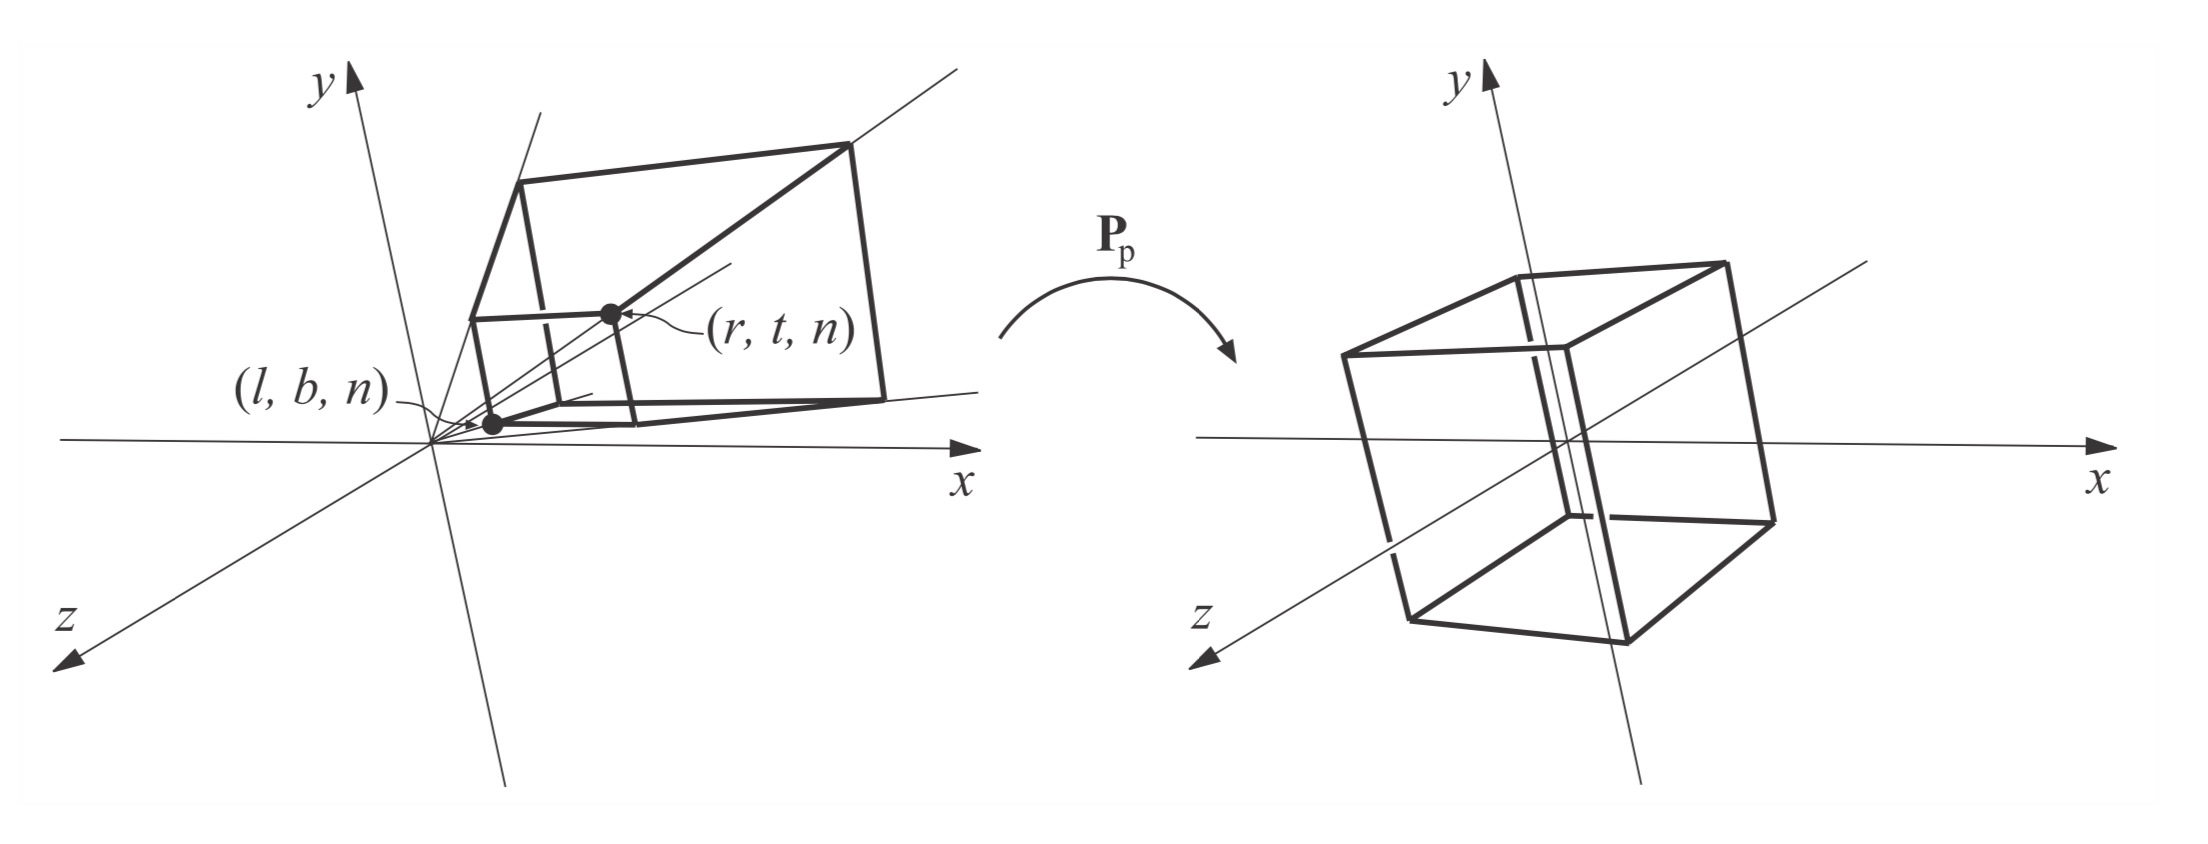
\includegraphics[width=1.0\linewidth]{pic-3.jpg}
  \end{figure}	

  我们可以直观的看到,透视投影和正交投影的区别在于,透视投影实际上使用了一个视锥。它将一个视锥变换为了一个单位立方体。这样可以使得远处物品显得更为小。品行线在远处相交与无穷点。这正是我们人类观察世界的时候的真实模样。所以透视投影在3D图形学中有着重要的运用场景。

  其实推导透视投影矩阵可以有几种方法。这里我们着重讲述$2$种方法。推导方式不同主要是我们定义视锥的参数不同导致的,本质上是一回事。

  \subsection{The First}

  我们先来看看第一种推导方式,这里我们先来定义一个视锥。我们还是先看图片。通过图片来看视锥的基本定义参数。

  \begin{figure}[htbp]
    \centering
    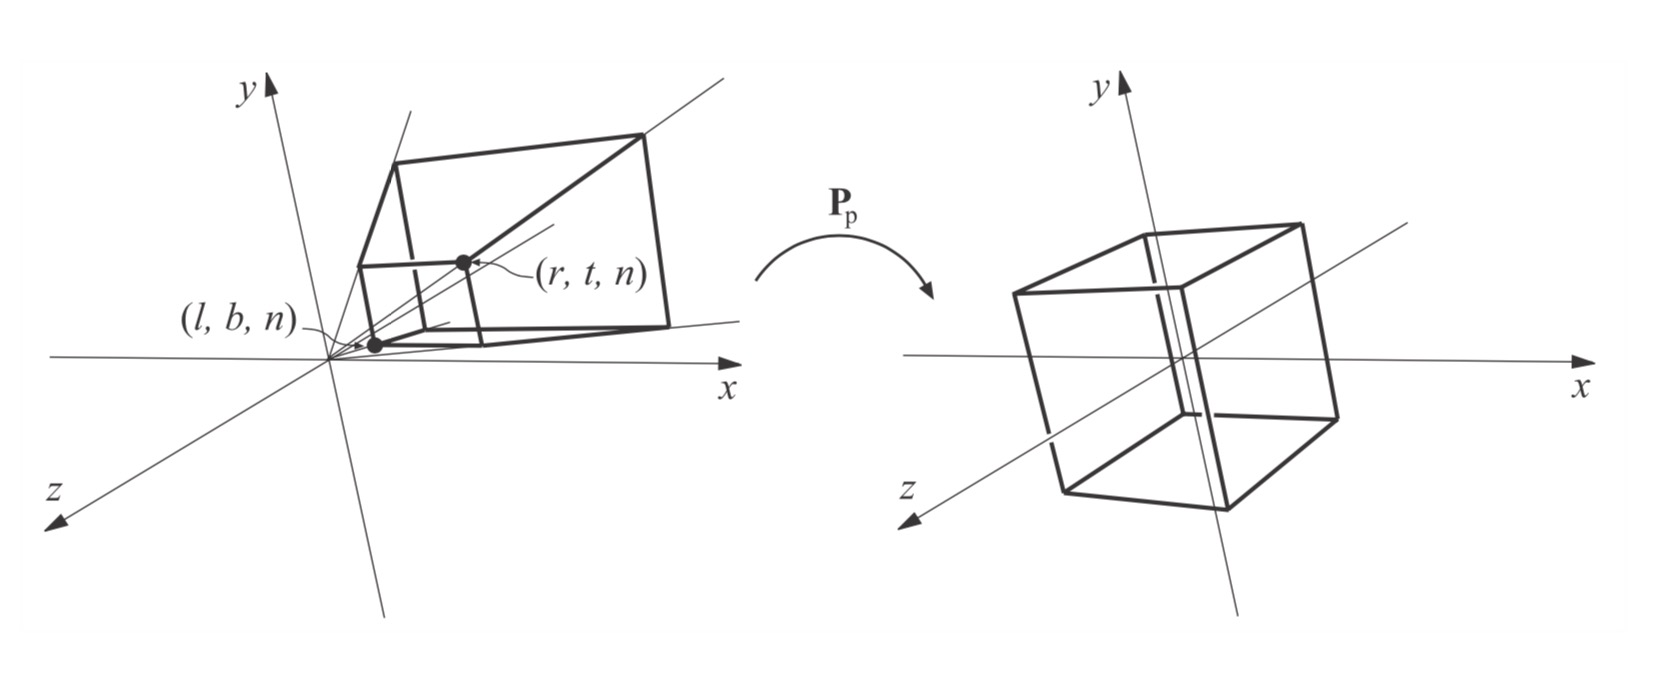
\includegraphics[width=1.0\linewidth]{pic-4.jpg}
  \end{figure}

  \subsubsection{定义视锥}

  这里我们依然定义$(l_x,b_y,n_z), (r_x,t_y,n_z)$,再另外定义$f_z$,这个定义和正交投影是不同的。我们没有定义$f_z$平面的范围。因为$f_z$的平面是由远点发射射线到$n_z$的四个角然后到达$f_z$所形成的平面。

  \subsubsection{如何推导透视矩阵}

  这里要做的就是把视锥里面的点映射到一个长度为$x\in[-1,1],y\in[-1, 1], z\in [-1,1]$的正方体区域$A$。下面我们来看一步步怎么做到的。
  
  \begin{equation}
    \label{eq:volume}
    A=\{(x,y,z)|x,y,z\in [-1,1]\}
  \end{equation}

  我们在这里列出一张辅助图像作为帮助希望读者更好理解,下面的计算过程。

  \begin{figure}[htbp]
    \centering
    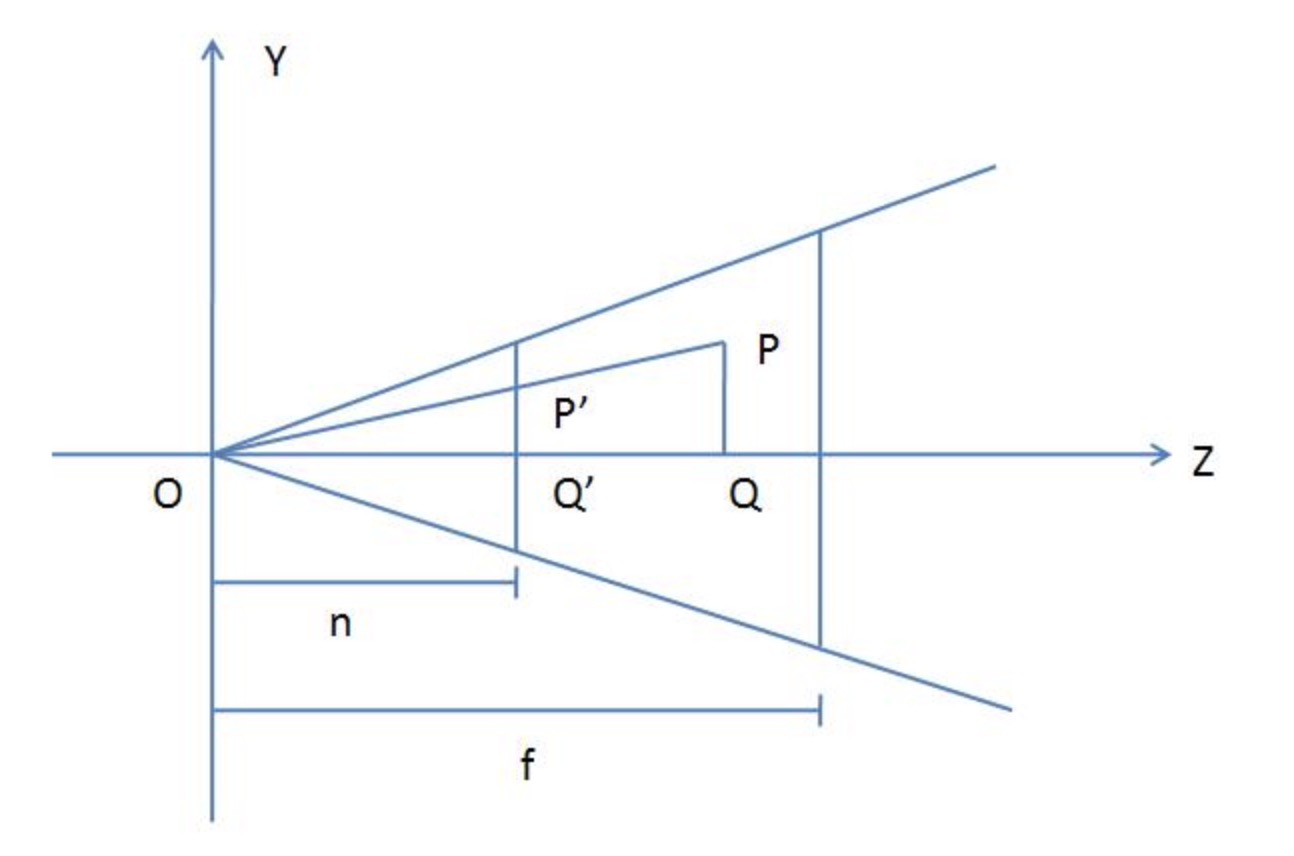
\includegraphics[width=0.8\linewidth]{pic-5.jpg}
  \end{figure}	

  \begin{itemize}
  \item 将视锥中的一个点$P=(P_x,P_y,P_z)$投影到$n_z$屏幕上的一点$(x,y)$。这个怎么计算呢?实际上就是计算$(0,0,0)$到$P$点之间的直线与$n_z$的交点。
    \begin{equation}
      \label{eq:nplane}
      x=-\frac{n}{P_z}P_x,y=-\frac{n}{P_z}P_y
    \end{equation}
  \item 接下来再将$x,y$压缩到$x^{'}\in [-1,1],y^{'}\in [-1,1]$内。

    \begin{equation}
      \label{eq:iden}
      \left.
        \begin{aligned}
          x^{'}=(x-l)\frac{2}{r-l}-1\\
          y^{'}=(x-b)\frac{2}{t-b}-1
        \end{aligned}
      \right.
    \end{equation}

    我们现在把等式\eqref{eq:nplane}带入\eqref{eq:iden}中可得

    \begin{equation}
      \label{eq:xy}
      \left.
        \begin{aligned}
          x^{\prime}=\frac{2 n}{r-l}\left(-\frac{P_{x}}{P_{z}}\right)-\frac{r+l}{r-l}\\
          y^{\prime}=\frac{2 n}{t-b}\left(-\frac{P_{y}}{P_{z}}\right)-\frac{t+b}{t-b}
        \end{aligned}
      \right.
    \end{equation}

    至此我们解决了将视锥中的点$P$的$P_x,P_y$坐标映射到了区域\eqref{eq:volume}中。
  \item 现在我们来解决将$P$中的$P_z$映射到区域\eqref{eq:volume}中。$P_z$的映射相对简单一些。
    \begin{equation}
      \label{eq:z}
      z^{\prime}=-\frac{2 n f}{f-n}\left(-\frac{1}{P_{z}}\right)+\frac{f+n}{f-n}
    \end{equation}
  \end{itemize}

  至此我们可以根据\eqref{eq:xy},\eqref{eq:z},可以得到如下等式。

  \begin{equation}
    \label{eq:xyz}
    \left.
      \begin{aligned}
        -x^{\prime} P_{z}&=\frac{2 n}{r-l} P_{x}+\frac{r+l}{r-l} P_{z}\\
        -y^{\prime} P_{z}&=\frac{2 n}{t-b} P_{y}+\frac{t+b}{t-b} P_{z}\\
        -z^{\prime} P_{z}&=-\frac{f+n}{f-n} P_{z}-\frac{2 n f}{f-n}
      \end{aligned}
    \right.
  \end{equation}

  由此我们就可以根据\eqref{eq:xyz}写出我们的透视投影矩阵为

  \begin{equation}
    \label{eq:proj}
    \mathbf{P}^{\prime}=\mathbf{M}_{\text { fustum }} \mathbf{P}=
    \left[
      \begin{array}{cccc}
        {\frac{2 n}{r-l}} & {0} & {\frac{r+l}{r-l}} & {0} \\
        {0} & {\frac{2 n}{t-b}} & {\frac{t+b}{t-b}} & {0} \\
        {0} & {0} & {-\frac{f+n}{f-n}} & {-\frac{2 n f}{f-n}} \\
        {0} & {0} & {-1} & {0}
      \end{array}\right]
    \left[
      \begin{array}{c}{P_{x}} \\
        {P_{y}} \\
        {P_{z}}
        \\ {1}
      \end{array}
    \right]
  \end{equation}

  最终我们得到的这个矩阵就是透视投影矩阵。如果我们$f\rightarrow \infty$ 那么还可以得到

  \begin{equation}
    \label{eq:projinf}
    \mathbf{M}_{\text { infinite }}=\lim _{f \rightarrow \infty} \mathbf{M}_{\text { frustum }}=\left[\begin{array}{cccc}{\frac{2 n}{r-l}} & {0} & {\frac{r+l}{r-l}} & {0} \\ {0} & {\frac{2 n}{t-b}} & {\frac{t+b}{t-b}} & {0} \\ {0} & {0} & {-1} & {-2 n} \\ {0} & {0} & {-1} & {0}\end{array}\right]
  \end{equation}

  \subsection{The Second}

  接下来,我们来看看另外一种推导方式。当然我们的视锥的定义会略有不同。
  
  \subsubsection{定义视锥}

  这里介绍的第二种定义视锥的方法,的基本原理如下图。
  \begin{figure}[htbp]
    \centering
    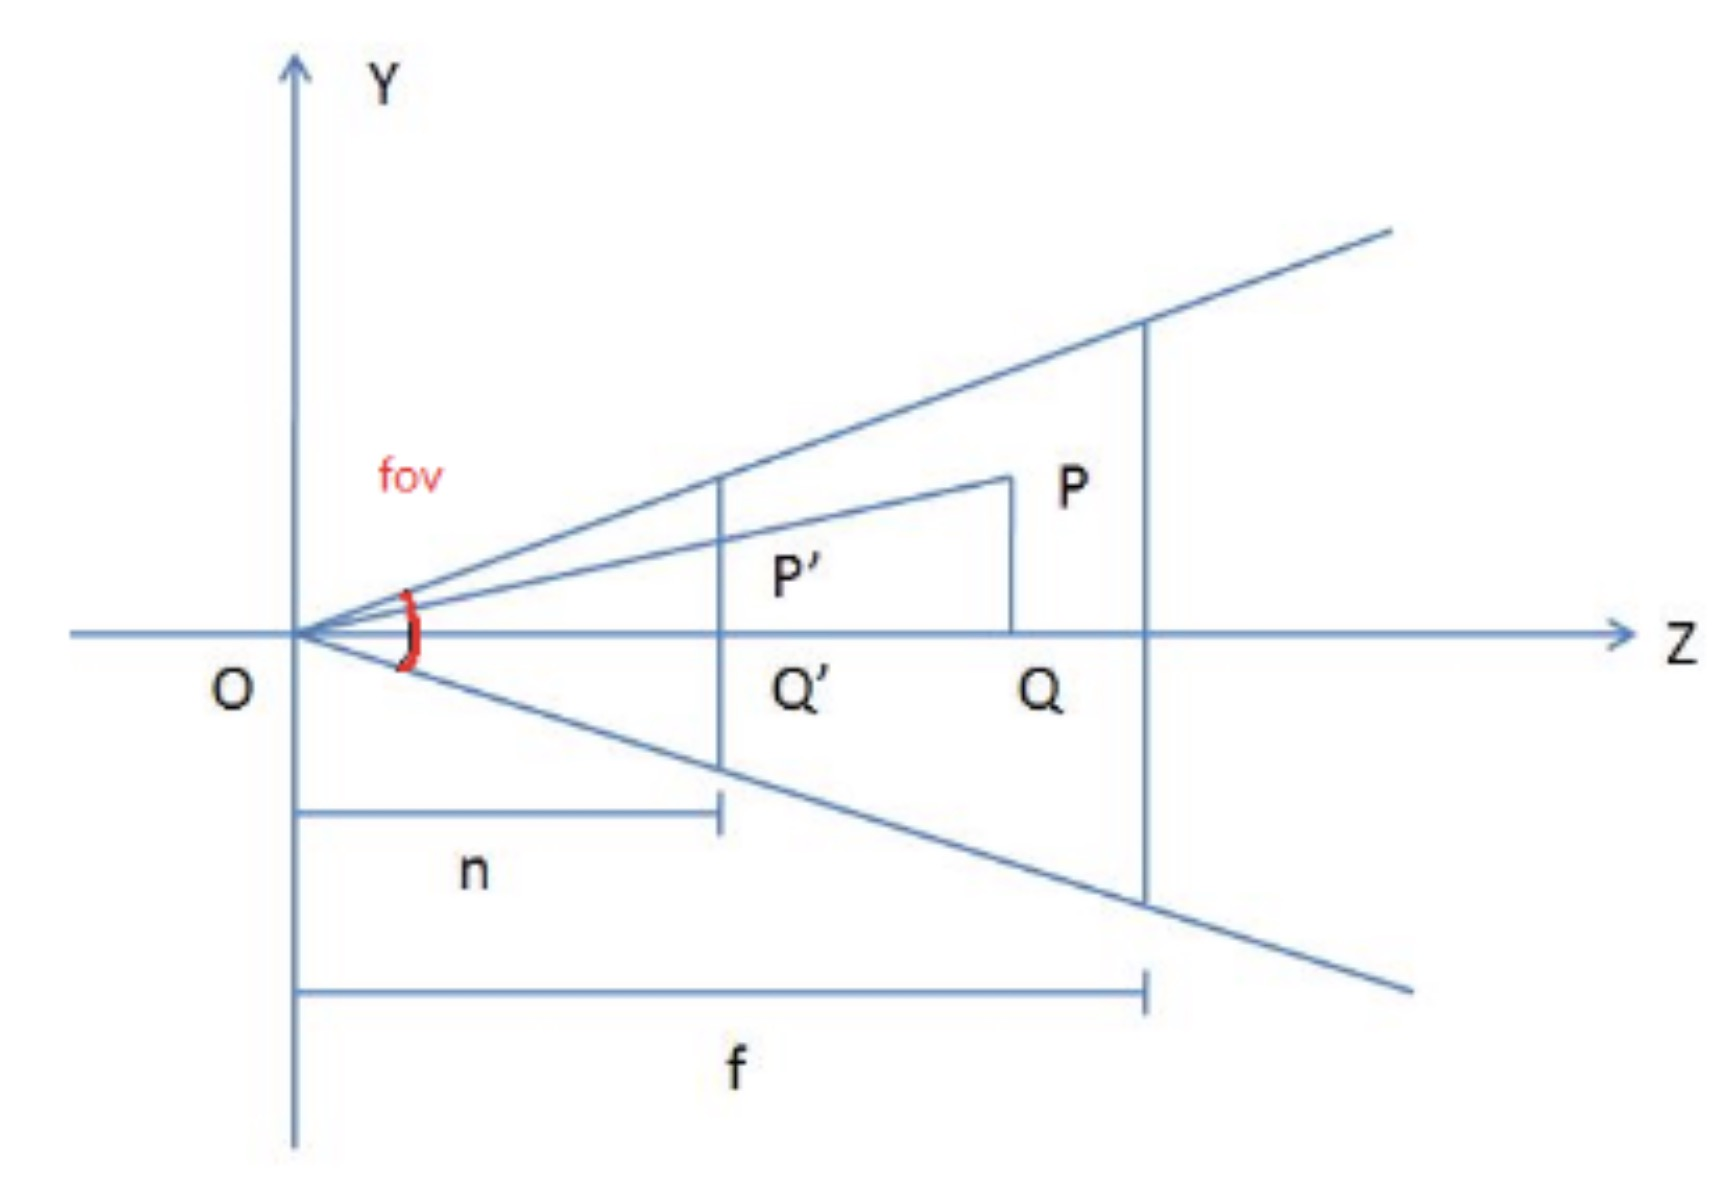
\includegraphics[width=0.6\linewidth]{pic-6.jpg}
  \end{figure}

  其中的参数为
  \begin{itemize}
  \item \textbf{FOV}, field of view.纵向的视角大小。
  \item aspect:裁剪面的宽高比
  \item zNear:近裁剪面离摄像机的距离,图中的n
  \item zFar:远裁剪面离摄像机的距离,图中的f    
  \end{itemize}

  通过以上的数据,我们可以唯一的确定一个透视投影矩阵。注意,这种定义方法和前面的定义方法没有什么本质的不同。他们之间只有一点微妙的区别。等一下我会详细来讲解,这个微妙的区别。我们等会就不会完整的再推到一次透视投影矩阵,而是将第二种方法的参数和第一种方法的参数进行映射。直接写出透视投影矩阵。现在我们来看看具体怎么做。

  我们这里有2个新的参数一个是\textbf{FOV},一个是 aspect.我们下面要做的就是使用前面的第一种定义方法来表示这两个参数
  \begin{itemize}
  \item \textbf{FOV},我们假设\textbf{FOV},的角度为$\theta$,那么我们可以很容易得到
    \begin{equation}
      \label{eq:fov}
      cot(\theta/2)=\frac{n}{(t-b)/2}
    \end{equation}
  \item aspect
    \begin{equation}
      \label{eq:aspect}
      aspect = \frac{r-l}{t-b}
    \end{equation}
  \end{itemize}

  把\eqref{eq:fov},\eqref{eq:aspect},代入\eqref{eq:proj},可得

  \begin{equation}
    \label{eq:proj_fov}
        \mathbf{P}^{\prime}=\mathbf{M}_{\text { fustum }} \mathbf{P}=
    \left[
      \begin{array}{cccc}
        {cot(\theta/2)/aspect} & {0} & {\frac{r+l}{r-l}} & {0} \\
        {0} & {cot(\theta/2)} & {\frac{t+b}{t-b}} & {0} \\
        {0} & {0} & {-\frac{f+n}{f-n}} & {-\frac{2 n f}{f-n}} \\
        {0} & {0} & {-1} & {0}
      \end{array}\right]
    \left[
      \begin{array}{c}{P_{x}} \\
        {P_{y}} \\
        {P_{z}}
        \\ {1}
      \end{array}
    \right]
  \end{equation}

  \textbf{微妙的区别},这个区别在于什么,注意看矩阵的$M_{1,3},M_{2,3}$项,他们依然存在。为什么?因为在第一种方法中$|r|$可以不等于$l$, $|t|$也可以不等于$|b|$,所以会出现$M_{1,3},M_{2,3}$,但是我们的第二种定义其实默认承认了$r=-l,t=-b$,因为我们只定义\textbf{FOV}和\textbf{aspect},所以只能是$r=-l,t=-b$.最终,$M_{1,3}=0,M_{2,3}=0$

  \begin{equation}
    \label{eq:proj_fov_final}
        \mathbf{P}^{\prime}=\mathbf{M}_{\text { fustum }} \mathbf{P}=
    \left[
      \begin{array}{cccc}
        {cot(\theta/2)/aspect} & {0} & {0} & {0} \\
        {0} & {cot(\theta/2)} & {0} & {0} \\
        {0} & {0} & {-\frac{f+n}{f-n}} & {-\frac{2 n f}{f-n}} \\
        {0} & {0} & {-1} & {0}
      \end{array}\right]
    \left[
      \begin{array}{c}{P_{x}} \\
        {P_{y}} \\
        {P_{z}}
        \\ {1}
      \end{array}
    \right]
  \end{equation}

  这就是我们的第二种透视投影的定义方法。

  \subsection{透视总结}

  我们可以看到我们定义了两种透视投影方法,第一种明显要比第二种的透视投影种类多。因为第二种的约束条件更强。所以第二种方式能表示的透视投影矩阵的种类就越小。总体来看我们可以得到

  \begin{displaymath}
    N_{\mbox{第二种方法}} \subset N_{\mbox{第一种方法}}
  \end{displaymath}

  \section{投影矩阵推导总结}

  本文应该清晰的推导出来了两种投影矩阵,一种是正交投影,一种是透视投影。透视投影矩阵本文提出了两种方法。其中第二种方法实际上是第一种方法的一个子集。希望大家能够通过阅读本文,愉快的了解和学习投影矩阵的细节。
  
\end{CJK}
\end{document}
